\chapter{Ein- und mehrstellige Funktionen}

Funktionen oder Abbildungen sind die wesentlichen mathematischen Objekte, die in der Analysis und Infinitesimalrechnung untersucht werden. Sie sind deshalb auch von besondere praktischer Bedeutung, da sich mit ihnen Zusammenhänge in den Naturwissenschaften modellieren lassen. Solche Zusammenhänge der realen Welt sind meist komplex, eine untersuchte Größe hängt meist nicht nur von einem, sondern von vielen Faktoren ab. Etwa hängt der elektrische Widerstand von Spannung und Stromstärke ab, der Luftdruck von drei Raum- und einer Zeitkoordinaten. Dementsprechend definiert man auch sogenannte mehrstellige Funktionen, welche mehr als ein Argument aufweisen. In diesem Kapitel werden wir zuerst den Funktionsbegriff näher definieren und anschließend einige ausgewählte wichtige Eigenschaften von Funktionen beleuchten.

\section{Funktionsbegriff}

\begin{definition}{Begriff der Funktion}{Function}
    Eine \textbf{Funktion} $f$ ist eine eindeutige Abbildung beziehungsweise Zuordnung von Elementen einer Grundmenge $\mathbb{S}$ zu Elementen einer Bildmenge $\mathbb{C}$. Die Elemente der Grundmenge heißen \textbf{Argumente}, die Elemente der Bildmenge \textbf{Funktionswerte}. Eindeutigkeit meint hierbei, dass keinem Argument mehr als ein Funktionswert zugeordnet ist.

    Wird jedem Argument ein Funktionswert zugeordnet, spricht man von einer \textbf{totalen Funktion}. Besteht die Zuordnung nur für manche Argumente, spricht man von einer \textbf{partiellen Funktion}. Die Menge $\mathbb{D} \subseteq \mathbb{S}$, für die ein Funktionswert erklärt ist, heißt Definitionsbereich.

    Man schreibt: $f: \mathbb{S} \to \mathbb{C}$.
\end{definition}

Diese Definition macht noch keine Aussage darüber, von welcher Art die Elemente sind. Wählt man reelle Zahlen als Elemente, erhält man die aus der Schulmathematik bekannten reellwertige Funktion. Es können aber auch Abbildungen anderer Elemente betrachtet werden. Beispielsweise werden in der Booleschen Algebra logische Verknüpfungen (\emph{and}, \emph{or}) als Abbildung zwischen Wahrheitswerten (\emph{true}, \emph{false}) betrachtet. Der Differentialoperator ist eine Abbildung auf Funktionen, die einer Funktion ihre Ableitung zuweist.

An dieser Stelle noch eine wichtige Anmerkung. Der mathematische Funktionsbegriff darf nicht mit dem Funktionsbegriff in der Programmierung verwechselt werden. Eine mathematische Funktion ist deterministisch in dem Sinne, das der Rückgabewert vollständig vom Ein- oder Übergabewert abhängt. Dies ist in der Programmierung nicht üblich -- dort kann der Rückgabewert etwa auch von globalen Konstanten, Umgebungsvariablen, Input-Operationen oder bei Methoden in der objektorientieren Programmierung auch vom aktuellen Zustand des Objekt abhängen. Weiterhin sind mathematische Funktionen pur, sie liefern einen Wert zurück und machen sonst nichts. Andererseits können Funktionen in der Programmierung noch sogenannten \emph{Seiteneffekte} aufweisen, etwa das Senden eines \mention{Http}-Requests, das Modifizieren eines Zustands, oder das Schreiben von Log-Ausschriften. Ein Programmier-Paradigma, dass sich stark an mathematischen Funktionen anlehnt, ist die \emph{funktionale Programmierung}.

\begin{example}{Definitionsbereich und Wertebereich}{DomainCodomain}
    Durch die Zuweisung $x\mapsto\frac{1}{x}$ ist eine Abbildung $f: \R \to \R$ zwischen reellen Zahlen definiert. Für die Zahl $0$ ist keine Zuordnung möglich, da hier der Ausdruck $1/0$ nicht erklärt ist. Es handelt sich also um eine partielle Funktion mit dem Definitionsbereich $\mathbb{D} = \lbrace x \in \R | x \ne 0 \rbrace = \R \setminus \lbrace 0 \rbrace$. Außer der $0$ kann jeder Funktionswert angenommen werden, mithin lautet der Wertebereich ebenfalls $\mathbb{C} = \R \setminus \lbrace 0 \rbrace$.
\end{example}

Unabhängig der Art der Elemente besteht eine Möglichkeit zur Veranschaulichung von Funktionen in der Darstellung als Wertetafel oder Pfeildarstellung wie in Abbildung \ref{fig:FunAsArrows}. Links in der Abbildung ist eine Funktion $f: \N \to \N$ dargestellt, die jeder natürlichen Zahl ihre Quadratzahl zuweist. Rechts ist der boolesche Operator \emph{Exklusives Oder} abgebildet, der eine Funktion zwischen einem Paar von Wahrheitswerten zu einem Wahrheitswert ist.

\begin{figure}[h]
    \caption{Darstellung von Funktionen als Pfeildiagramm}
    \label{fig:FunAsArrows}
    \centering
    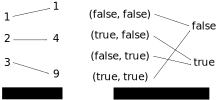
\includegraphics[width=0.8\textwidth]{./svg/function-as-arrows.png}
\end{figure}

Für diese Vorlesung beschränken wir uns auf Funktionen zwischen reellen Zahlen. Hier unterscheiden wir zwei Arten, je nachdem, ob der Funktionswert nur von einer reellen Zahl oder von mehreren abhängt.

\begin{definition}{Einstellige Funktion}{UnivarFun}
    Von einer \textbf{einstelligen reellwertigen Funktion} spricht man, wenn eine Abbildung $f: \R \to \R$ von einer reellen Zahl zu einer anderen reellen Zahl vorliegt.
\end{definition}

\begin{definition}{Mehrstellige Funktion}{MultivarFun}
    Von einer \textbf{$n$-stelligen reellwertigen Funktion} spricht man, wenn eine Abbildung $f: \R^n \to \R$ von einer Tupel reeller Zahlen zu einer anderen reellen Zahl vorliegt.
\end{definition}

Der Gewinn beim Verkauf eines Produkts in Abhängigkeit der produzierten Stückzahl stellt ein Beispiel für eine einstellige Funktion dar und könnte etwa $f: x \to 0.2\text{Euro} \cdot x - 200\text{Euro}$ lauten (20 Cent Gewinn pro verkauften Produkt, 200  Fixkosten für Miete). Der elektrische Widerstand eines Drahtes in Abhängigkeit seiner Länge, seiner Querschnittsfläche und seines Materials wird dargestellt durch eine dreistellige Funktion und lautet $R: (l, A, \rho) \to \rho \frac{l}{A}$.

Neben dem Pfeildiagramm gibt es auch weitere Möglichkeiten, ein- und mehrstellige Funktionen graphisch darzustellen.

\begin{definition}{Graph einer Funktion}{FunGraph}
    Der Graph $G$ einer n-stelligen Funktion $f: \R^n \to \R$ ist die Menge aller $(n+1)$-dimensionalen Punkte, die einem Argument-Funktionswerte-Paar entsprechen.

    $$
    G = \lbrace (p_1, p_2, ..., p_{n+1}) \in R^{n+1} | f((p_1, ..., p_n)) = p_{n+1} \rbrace
    $$

    Dieser Graph kann in einem $(n+1)$-dimensionalen kartesischen Koordinatensystem veranschaulicht werden.
\end{definition}

Für einstellige Funktionen ist der Graph zweidimensional und in einem $x-y$-Koordinatensystem wie in Abbildung \ref{fig:GraphUnivarFun} gut überschaubar. Für zweistellige Funktionen benötigt man bereits ein dreidimensionalen Koordinatensystem, in dem die Form des Graphen bereits schwerer zu überschauen ist, da der Graph meist auf eine zweidimensionale Bildschirmebenene projiziert wird. Drei- und mehrstellige Funktionen sind auf diese Weise nur kaum bis gar nicht zur veranschaulichen. Die meisten Beispiele dieser Vorlesung werden sich daher auf ein- und zweidimensionale Funktionen beschränken. In Abbildung \ref{fig:GraphUnivarFun} ist der Graph einer einstelligen Funktion dargestellt. Abbildung \ref{fig:GraphMultivarFun} zeigt den Graph einer zweistelligen Funktion aus vier verschiedenen Blickwinkeln. Man beachte hierbei besonders die Seitensicht: Wird eines der beiden Argumente konstant gehalten und nur das anderen variiert, erhält man eine einstellige Funktion. Je nachdem, auf welchem Wert man das eine Argument konstant hält, ergeben sich verschiedene Funktionen.

\begin{figure}[h]
    \caption{Graph einer einstelligen Funktion}
    \label{fig:GraphUnivarFun}
    \centering
    \includegraphics[width=0.8\textwidth]{./gnuplot/example-univariate-function.png}
\end{figure}

\begin{figure}[h]
    \caption{Graph einer zweistelligen Funktion}
    \label{fig:GraphMultivarFun}
    \centering
    \includegraphics[width=0.45\textwidth]{./gnuplot/example-multivariate-function-1.png}
    \includegraphics[width=0.45\textwidth]{./gnuplot/example-multivariate-function-2.png}
    \includegraphics[width=0.45\textwidth]{./gnuplot/example-multivariate-function-3.png}
    \includegraphics[width=0.45\textwidth]{./gnuplot/example-multivariate-function-4.png}
\end{figure}

Für zweistellige Funktionen gibt es auch noch weitere Darstellungsformen, die manchmal übersichtlichen und einfacher zu erfassen sind. Die erste Darstellungsweise, die sogenannte \emph{Konturdarstellung}, wird etwa bei Wanderkarten für Abbildung zweidimensionaler Punkte der Erdoberfläche zur Höhe über Normalnull verwendet. Die Höhe an jedem Punkt wird farbig markiert, Kurven gleicher Höhe werden mit einer Linie dargestellt (Höhenlinien).

\begin{definition}{Konturlinie einer mehrstelligen Funktion}{ContLine}
    Unter einer \textbf{Konturlinie} zur Konstanten $c$ einer n-stelligen Funktion $f: \R^n\to\R$ versteht man die Menge $L_c$ aller Punkte des Definitionsbereichs, an dem der Funktionswert gleich der Konstanten $c$ ist.

    $$
       L_c = \lbrace x \in \R^n | f(x) = c \rbrace
    $$
\end{definition}

\begin{example}{Konturlinien einer Funktion}{ContLine}
    Gesucht sind die Konturlinien der zweistelligen Funktion $f: (x,y) \to x^2+y^2$. Offensichtlich kann die Funktion keine negativen Werte annehmen. Wir bezeichnen die Konturlinienkonstante mit $R^2$. Nach Definition sind nun die Punkte $(x,y)\in\R^2$ gesucht, für die $x^2+y^2=R^2$ gilt. Unter Beachtung des Satzes von Pythagoras erkennen wir, dass es sich um alle Punkte handelt, deren Abstand zum Koordinatenursprung $R$ beträgt. Mithin handelt es sich bei den Konturlinien von $f$ also um zum Ursprung konzentrische Kreislinien. Diese sind in Abbildung \ref{fig:ExContLine} dargestellt.
\end{example}

\begin{figure}[h]
    \caption{Konturlinien der Funktion aus Beispiel \ref{ex:ContLine}}
    \label{fig:ExContLine}
    \centering
    \includegraphics[width=0.95\textwidth]{./gnuplot/example-contour-plot.png}
\end{figure}

Als zweite Darstellungsform gibt es noch das sogenannte Gradientenfeld, wobei durch Pfeile angezeigt wird, in welcher Richtung die Funktionswert am stärksten zunehmen. Dies ist etwa bekannt aus Wetterkarten, wo die Windrichtung (näherungsweise) als Gradient des Luftdruckes eingezeichnet ist.

\begin{definition}{Gradientenfeld einer zweistelligen Funktion}{GradField}
    Unter dem Gradientenfeld einer $n$-stelligen Funktion $f: \R^n \to R$ versteht man die Funktion $G_f: \R^n \to \R^n$, welche jedem Punkt $\vec{r}=(x_1,x_2,...,x_n)$ des Definitionsbereichs von $f$ eine Richtung (einen $n$-dimensionalen Vektor) zuordnet, welcher in Richtung des stärksten Anstiegs von $f$ im Punkt $\vec{r}$ zeigt.

    $$
        G_f(\vec{r}) = \vec\nabla f(\vec{r}) = \rvec{\pdd{f}{x_1}(\vec{r})}{\vdots}{\pdd{f}{x_n}(\vec{r})}
    $$
\end{definition}

\begin{example}{Konturlinien einer Funktion}{GradField}
    Gesucht ist das Gradientenfeld der zweistelligen Funktion $f: (x,y) \to x^2+y^2$. Gemäß Definition müssen wir zuerst die beiden partiellen Ableitungen nach $x$ und $y$ berechnen:

    \begin{alignat*}{1}
        \pdd{}{x} x^2+y^2 &= 2x \\
        \pdd{}{y} x^2+y^2 &= 2y
    \end{alignat*}

    Damit lässt sich das Gradientenfeld $G: \R^2 \to \R$ nun angeben als:

    $$
        G(x,y) = \tvec{2x}{2y}
    $$

    Die Richtung des stärksten Anstiegs verläuft wie in Abbildung \ref{fig:ExGradField} zu sehen also immer radial weg vom Koordinatenursprung. Aus der Anschauung ist dies unmittelbar klar, bei dem Graphen von $f$ handelt es sich um einen nach oben geöffnete Kesselform.
\end{example}

\begin{figure}[h]
    \caption{Gradientenfeld der Funktion aus Beispiel \ref{ex:GradField}}
    \label{fig:ExGradField}
    \centering
    \includegraphics[width=0.65\textwidth]{./gnuplot/example-gradient-field.png}
\end{figure}

An dieser Stelle noch eine kurze Anmerkung zum sogenannten \emph{Feld}. Speziell in der Physik bezeichnet man mit einem Feld eine Größe, welche an jedem Punkt des Raums einen anderen Wert haben kann. Diese stellen mehrstellige Funktionen dar. Etwa ist der Luftdruck ein Feld, wo jedem Raumpunkt ein Luftdruckwert zugeordnet wird. Da der Luftdruck nur ein einzelne Zahl (=Skalar) ist, nennt man solche Felder auch skalare Felder. Das elektrische Feld ist ein vektorielles Feld und weist jedem Raumpunkt einen Vektor (Richtung und Betrag) zu, der angibt, welche Kraft eine geladene Masse an diesem Raumpunkt erfährt.

\section{Spezielle Funktionen}

Grundfunktionen
Polynome
Gebrochenrat. Fkt.
Transformationen (Verschiebung, Skalierung)
Verkettung

\section{Eigenschaften von Funktionen}
Stetigkeit, stetige Erägnzung

Monotonie, Injektiv, Surjektiv, Bijektiv, Umkehrfkt.

Symmetrie Periodizität

Globale Extreme, Lokale Extrema
